\documentclass[a4paper]{article}
\usepackage[utf8]{inputenc}
\usepackage[brazil]{babel}

% Referências no estilo ABNT
% Usar no R 'citation()' para citar o R ou pacotes
%\usepackage[alf]{abntex2cite}
%\usepackage[alf, abnt-emphasize=bf]{abntcite}
\usepackage{natbib}


\usepackage{geometry}
\geometry{a4paper, left=40mm, right=40mm, top=25mm, bottom=25mm}

% Cores: http://latexcolor.com/.
\usepackage{xcolor}
\definecolor{ballblue}{rgb}{0.13, 0.67, 0.8}
\newcommand{\tc}[1]{\textcolor{ballblue}{#1}}

\usepackage{graphics}
\usepackage{hyperref}
\usepackage{float}
\hypersetup{colorlinks = true}

\title{Análise do Clima em Colombo para o período \tc{30/01/2018} a \tc{08/02/2018}}
\author{Acadêmico Jayme Gomes dos Santos Junior}
\date{}

\usepackage{Sweave}
\begin{document}
\Sconcordance{concordance:Sabatina_clima.tex:Sabatina_clima.Rnw:%
1 22 1 1 26 5 1 1 0 11 1 1 4 1 2 2 1 1 24 21 0 1 15 5 1 1 4 1 3 18 1}


%\bibliographystyle{abnt-alf}
%\bibliographystyle{plainnat}
\maketitle

Este relatório utiliza os dados climáticos da cidade de Colombo no período de \tc{10} dias compreendidos entre \tc{30/01/2018} e \tc{08/02/2018}.

 \tc{O dia com maior precipitação no período foi 07/02/2018 com precipitação de 3.8mm}, como mostra a figura\ref{plot}.

\begin{figure}[h]
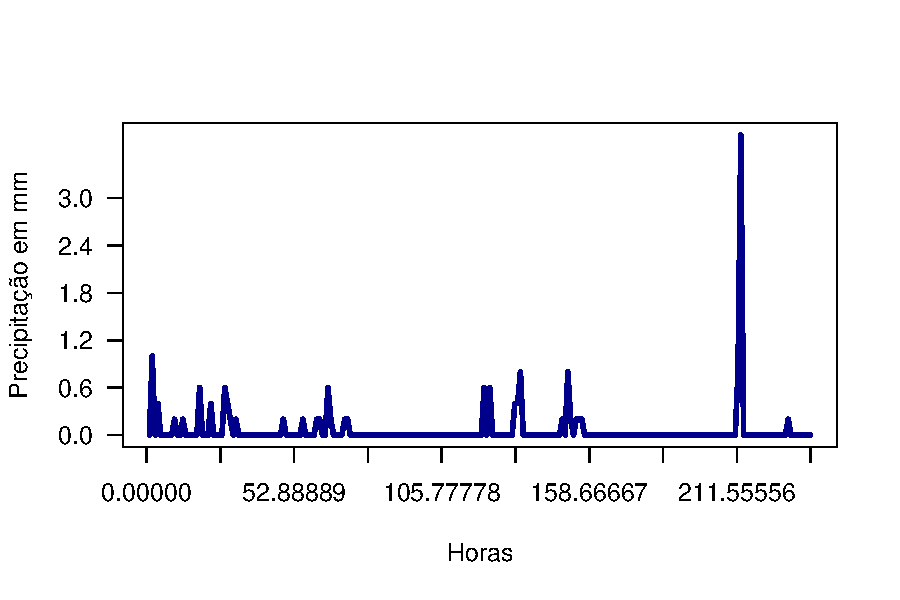
\includegraphics{Sabatina_clima-002}
\caption{Precipitação registrada a cada hora em Colombo.}\label{plot}
\end{figure}

% latex table generated in R 3.4.2 by xtable 1.8-2 package
% Tue Mar 20 19:09:28 2018
\begin{table}[ht]
\centering
\begin{tabular}{rlrrr}
  \hline
 & Data & Temperatura.Média & Temperatura.Máxima & Temperatura.Mínima \\ 
  \hline
1 & 01/02/2018 & 17.84 & 23.80 & 13.90 \\ 
  2 & 02/02/2018 & 19.18 & 26.10 & 14.70 \\ 
  3 & 03/02/2018 & 18.45 & 25.50 & 11.00 \\ 
  4 & 04/02/2018 & 18.06 & 22.70 & 15.60 \\ 
  5 & 05/02/2018 & 18.15 & 24.00 & 15.20 \\ 
  6 & 06/02/2018 & 18.18 & 25.60 & 13.00 \\ 
  7 & 07/02/2018 & 18.57 & 26.20 & 14.70 \\ 
  8 & 08/02/2018 & 21.22 & 28.50 & 17.10 \\ 
  9 & 30/01/2018 & 17.42 & 21.60 & 15.30 \\ 
  10 & 31/01/2018 & 19.01 & 25.40 & 15.40 \\ 
   \hline
\end{tabular}
\caption{Mostra a temperatura média, máxima e mínima de cada dia do período} 
\label{xtable}
\end{table}
\tc{08/02/2018} foi o dia com a temperatura média mais alta, \tc{21.2208333333333}°C.
Já a temperatura mais baixa de todo o período foi \tc{11}°C no dia \tc{03/02/2018}
e a mais alta ocorreu no dia \tc{08/02/2018} alcançando \tc{28.5}°C.

\begin{figure}[H]
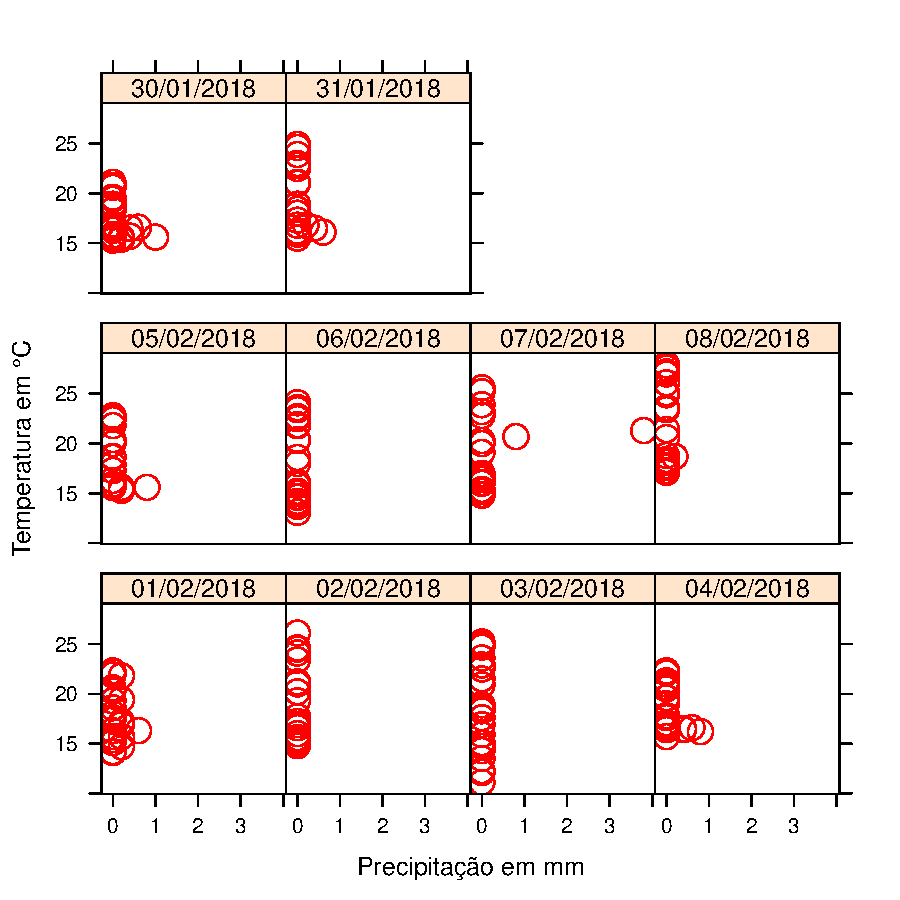
\includegraphics{Sabatina_clima-004}
\caption{Relação entre a temperatura e precipitação a cada dia.}\label{xyplot}
\end{figure}

Já na figura\ref{xyplot}, vemos a relação entre a temperatura e a precipitação em cada dia
do período.\\

Todo o relatório foi feito utilizando o R.\citep{r}\\

Na figura\ref{plot}, foi utilizado o pacote 'ggplot2'.\citep{ggplot2}\\

Na tabela\ref{xtable}, usou-se o pacote 'xtable'.\citep{xtable}\\

E o pacote 'lattice'\citet{lattice} para a figura\ref{xyplot}.\\

%Referências bibliográficas
\bibliographystyle{abbrvnat}
\bibliography{ref}

\end{document}
